\documentclass[12pt, a4paper]{article}

\usepackage[hmargin=2.5cm, vmargin=2cm]{geometry}
\usepackage{amsthm, amssymb, mathtools, yhmath, graphicx}
\usepackage{fontspec, type1cm, titlesec, titling, fancyhdr, tabularx}
\usepackage{color}
\usepackage{unicode-math}
\usepackage{float}
\usepackage{subfig}
\usepackage{hhline}
\usepackage{comment}
\usepackage[abbreviation,per-mode=symbol]{siunitx}
\usepackage{csvsimple}
\usepackage{subcaption}

\usepackage[CheckSingle, CJKmath]{xeCJK}
\usepackage{CJKulem}
\usepackage{enumitem}
\usepackage{tikz}
\usepackage[siunitx]{circuitikz}
\usepackage{wrapfig}
%\setCJKmainfont[BoldFont=cwTex Q Hei]{cwTex Q Ming}
%\setCJKsansfont[BoldFont=cwTex Q Hei]{cwTex Q Ming}
%\setCJKmonofont[BoldFont=cwTex Q Hei]{cwTex Q Ming}
\setCJKmainfont[BoldFont=cwTeX Q Hei]{cwTeX Q Ming}

\def\normalsize{\fontsize{12}{18}\selectfont}
\def\large{\fontsize{14}{21}\selectfont}
\def\Large{\fontsize{16}{24}\selectfont}
\def\LARGE{\fontsize{18}{27}\selectfont}
\def\huge{\fontsize{20}{30}\selectfont}

%\titleformat{\section}{\bf\Large}{\arabic{section}}{24pt}{}
%\titleformat{\subsection}{\large}{\arabic{subsection}.}{12pt}{}
%\titlespacing*{\subsection}{0pt}{0pt}{1.5ex}

\parindent=24pt

\DeclarePairedDelimiter{\abs}{\lvert}{\rvert}
\DeclarePairedDelimiter{\norm}{\lVert}{\rVert}
\DeclarePairedDelimiter{\inpd}{\langle}{\rangle}
\DeclarePairedDelimiter{\ceil}{\lceil}{\rceil}
\DeclarePairedDelimiter{\floor}{\lfloor}{\rfloor}

\newcommand{\unit}[1]{\:(\text{#1})}
\newcommand{\df}[1]{\mathop{}\!\mathrm{d^#1}}
\newcommand{\img}{\mathrm{i}}
\newcommand{\dD}{\mathrm{d}}
\newcommand{\dI}{\,\mathrm{d}}
\newcommand{\paral}{\mathbin{\|}}

\title{ \bf {\Huge 電子電路實驗3: VTC of CMOS Amplifier Circuits  }\\ 實驗結報}
\author{B02901178 江誠敏}

\begin{document}

\maketitle


\section{實驗結果}

\subsection{CMOS amplifier as an inverter}
\begin{center}
	\begin{tabular}{p{3cm}p{3cm}p{3cm}}
	\hline
	放大倍率 & 理論值 & 相對誤差 \\
	\hline 
	\hline
  $\SI{-20}{\volt \per \volt}$ & $\SI{-20}{\volt \per \volt}$ & $0.0\%$
  \end{tabular}
\end{center}

\subsection{CMOS analog circuit experiment (Resistance effect on the circuit)}
\begin{center}
	\begin{tabular}{p{3cm}p{3cm}p{3cm}}
	\hline
  電阻 & 放大倍率 \\
	\hline 
	\hline
  $\SI{20}\kohm$ & $\SI{-17}{\volt\per\volt}$ \\
  $\SI{510}\kohm$ & $\SI{-19}{\volt\per\volt}$ \\
  $\SI{1}\Mohm$ & $\SI{-20}{\volt\per\volt}$ \\
  $\SI{3.9}\kohm$ & $\SI{-20}{\volt\per\volt}$ \\
  $\SI{10}\kohm$ & $\SI{-20}{\volt\per\volt}$ \\
  \end{tabular}
\end{center}

\subsection{CMOS analog amplifier circuit experiment}

\begin{center}
	\begin{tabular}{p{3cm}p{3cm}p{3cm}}
	\hline
  電阻 & 電壓 \\
	\hline 
	\hline
  $v_{i(ac)}$ & $\SI{230}\mV$ \\
  $V_{i(dc)}$ & $\SI{3.68}\V$ \\
  $v_{o(ac)}$ & $\SI{3.48}\V$ \\
  $V_{o(dc)}$ & $\SI{4.14}\V$ \\
  \end{tabular}
\end{center}

\section{結報問題}

\begin{enumerate}[itemsep=20pt, topsep=10pt]

  \item {The $|V_{tn}| = |V_{tp}| = \SI{1}\V$, $K_n = 4K_p = \SI{100}{\micro\ampere\per\volt\squared}$
      in the circuit in Fig. 4, try to find: } \\[10pt]
    \begin{enumerate}[(a)]
      \item $V_D$ and $I_D$. \\
      答:\\
      First $V_{OV} = \SI{3}\V$ for both MOS.
      Since $K_n$ is $4$ times bigger than $K_p$, we thus guess that the NMOS is operating on
      triode mode. So we have
      \[ (\SI{100}{\micro\ampere}) V_D (3 - V_D / 2) + \frac{V_D - 4}{\SI{1}\Mohm} 
      = 0.5 (\SI{25}{\micro\ampere}) 3^2 \]
      Solve for $V_D$, we get $V_D \approx \boxed{\SI{0.416}\V}$, and our assumption that
      NMOS is operating on triode mode is correct since $\SI{0.416}\V < V_{OV} = \SI{3}\V$.
      Finally,
      \[ I_{Dp} = 0.5 \cdot 25 \cdot 3^2 = \boxed{\SI{112.5}{\micro\ampere}}, \quad 
        I_{Dn} = 100 \cdot V_D \cdot (3 - V_D/2) \approx \boxed{\SI{116.1}{\micro\ampere}} \]
      \item The voltage gain $A_v$ and output resistance $R_o$ for the circuit if the small 
        signal output resistance in drain for NMOS and PMOS are infinity.  \\
      答:\\
        Now considering small signal, the equation becomes
        
        \[ (\SI{100}{\micro\ampere}) V_D (3 + v_i - V_D / 2) + \frac{V_D - 4 - v_i}{\SI{1}\Mohm} 
        = 0.5 (\SI{25}{\micro\ampere}) (3 - v_i)^2 \]

        By differentiating, we obtain
        \begin{multline*}
        (\SI{100}{\micro\ampere}) \frac{\partial V_D}{\partial v_i}  (3 + v_i - V_D / 2) +
           (\SI{100}{\micro\ampere}) V_D  \left(1 - \frac{\partial V_D}{\partial v_i} / 2\right) + \\
           \frac{1}{\SI{1}\Mohm} \left( \frac{\partial V_D}{\partial v_i} - 1 \right) 
        = - (\SI{25}{\micro\ampere}) (3 - v_i)
        \end{multline*}
        Evaluate at $v_i = 0$, we get
        \[
          A_v = \frac{\partial v_o}{\partial v_i} \biggr|_{v_i=0}  =
          \frac{\partial V_D}{\partial v_i} \biggr|_{v_i=0} \approx \boxed{\SI{-0.446}{\volt\per\volt}}
        \]

        $R_o$ is obviously $\boxed{\SI{1}\Mohm}$.
    \end{enumerate}

  \item {Try to find the voltage gain $A_v$ and output resistance of the circuit in Fig. 7 as the switch turn to a and b .
      (Hint: the trans-conductance and output resistance of PMOS and NMOS are $g_{mp}$ , $r_{op}$, $g_{mn}$, $r_{om}$
      respectively.) } \\[10pt]
    答:\\
    If the switch is turned to a, by using small signal model, we have
    \[ v_o = -v_i g_m \left( r_{on} \paral r_{op} \right) \quad \Rightarrow 
    \quad A_v = \boxed{-g_{mn} \left( r_{on} \paral r_{op} \right)}\]
    If the switch is turned to b, using small signal model again, we have
    \[ v_o = -v_i g_m \left( r_{on} \paral r_{op} \right) \quad \Rightarrow 
    \quad A_v = \boxed{-(g_{mn} + g_{mp}) \left( r_{on} \paral r_{op} \right)}\]

  \item {利用NMOS元件物裡結構圖推導在 triode 和 saturation 時的 $I_D$ 。} \\[10pt]
    答:\\
    我們必須先求出電壓 $V$ 在 channel 間的函數。假設其為 $V(x)$。首先電流密度和電場的關係為
    \[ J = \rho \mu E = \rho \mu \frac{\partial V}{\partial x} \] 
    並且 channel 的高度 $h$ 和 $V$ 的關係為
    \[ -C_{ox} (V_{ov} - V) = \rho h \]
    我們假設 $\rho$ 是均勻的,因此有
    \[ I = J A = J h W = \rho h \mu \frac{\partial V}{\partial x} W = 
     -C_{ox} (V_{ov} - V) \mu \frac{\partial V}{\partial x}\]
    但 $I$ 必須與 $x$ 無關,否則會有電荷累積,解此微分方程,得
    \[ (V_{ov} - V)^2 = \alpha^2 - \frac{2 I L}{C_{ox} W \mu} \]
    代入 $x = 0, V(0) = 0$ 可得 $\alpha = V_{ov}$。最後代入 $x = L, V(L) = V_{GS}$,有
    \begin{align*}
      & (V_{ov} - V_{GS})^2 = V_{ov}^2 - \frac{2 I L}{C_{ox} W \mu} \\
      \Rightarrow & I = C_{ox} \mu \frac{W}{L} V_{ov} (V_{ov} - V_{GS}/2)
    \end{align*}

    但當 $V_{GS} > V_{ov}$ 時, 由 $ -C_{ox} (V_{ov} - V) = \rho h $ 會發現在末端的 $h$ 是
    負的\footnote{這裡 $\rho < 0$}! 事實上在這樣的情況,會有一點 $L'$ 使得 $V(L') = V_{ov}$,
    並且 $V(x) \equiv V_{ov}, \; \forall x,  L' \leq x \leq L$。此時上述的公式仍可使用,但應將
    $L \leftarrow L', \; V_{GS} \leftarrow V_{ov}$。一般將其近似為
    \[I = C_{ox} \mu \frac{W}{L} V_{ov}^2 \left( 1 + \frac{V_{GS}}{V_{A}} \right) \]
    
  \item {畫出NMOS與PMOS的$I_D-V_{DS}$曲線} \\[10pt]
    答:\\
    \begin{figure}[H]
    \begin{center}
      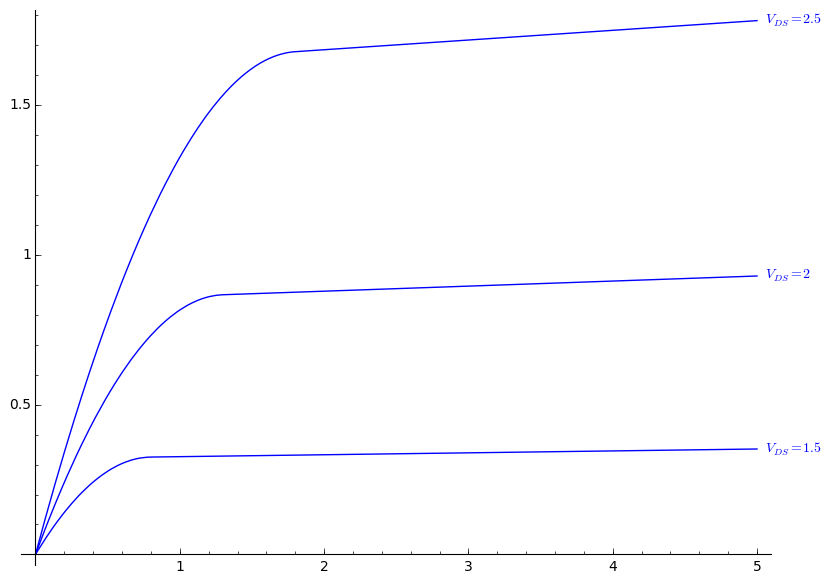
\includegraphics[width=0.7\textwidth]{p1.png}
    \end{center}
    \caption{}
    \end{figure}

  \item {請說明body effect,此效應的存在是好還是不好?請說明原因。} \\[10pt]
    答:\\
    Body effect 是因為通常在實際的應用上,所有 MOS 的 Base 都會被接在一起,而非和他的
    Source 端接在一起,導致 Threshold voltage $V_t$ 的改變,可用公式
    \[ V_t' = V_t + \gamma \left( \sqrt{V_{SB} + 2 \phi_B } - \sqrt{2 \phi_B} \right) \]
    描述。\\
    這樣的方式使 MOS circuit 在製造上比較容易,所有的 MOS 都在同一塊板上製造即可。
    並且通常 $V_t'$ 和 $V_t$ 的差距不會太大。 但在某些情況,$V_t'$ 的增加量不可被忽視,
    否則可能會導致元件的特性曲線偏離太多,並使整個電路失效。

\end{enumerate}

\section{心得}
這次的實驗慘慘的,因為我們做在邊疆地區,儀器都舊舊的,在 \texttt{X-Y} mode 下
居然還沒有 Cursor 可以用,害的我們只好狂調倍率,把倍率弄到超大,還是只能大概
抓一下數字。 不過有時候儀器不好,數據反而誤差更小。為什麼呢?因為沒有 cursor
所以只能大概估計一下,一估,好像永遠都是 $1:4$ ,在乘上原本的 $5$ 倍倍率,恰
恰好就是和參考值完全相同的 $20$ 倍,誤差 $0 \%$ ! 這個故事告訴我們有時候
我們身上有什麼不是重點,即使一無所有,運氣來了也是可以成為大贏家!
\end{document}

